\documentclass{article}
\usepackage[top=2.54cm, bottom=2.54cm, left=2.54cm, right=2.54cm]{geometry}
\usepackage{graphicx}
\setlength{\parskip}{12pt}
\setlength{\parindent}{0pt}
\begin{document}

\begin{center} Huilin Tong\\
ID:1261574
\end{center}

{\bf Discussion}\\

\begin{enumerate}
\item 
\begin{center}
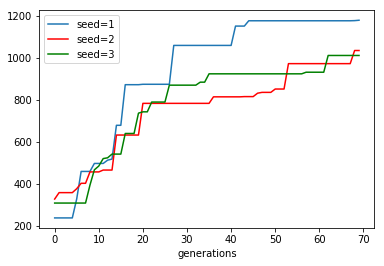
\includegraphics[scale=0.7]{d1.png}

Fig.1 Best distance vs. generation
\end{center}

\item Compare the best distance of such three situation with a certain generation. They're not identical since different seed() means it will differ when you choose the random number in this three cases.

\item Good initial solution:

0 0 0 0 1 |100 100 100 100

1 0 0 0 0 |0   0   0   0

This makes Manduca move fastest.

\item 210 generation is better. More generations means more diversity and more probability to get the optimal solution. Not definitely better since you probability falls on a local optimum and mutation and mate alone can not help out such local solution.
\end{enumerate}
\end{document}